% --------------------------------------------------
% DOCUMENT CLASS
% --------------------------------------------------

\documentclass[../quali_slides.tex]{subfiles}

\begin{document}

% --------------------------------------------------
% SLIDE
% --------------------------------------------------

\section{Regional NK DSGE Model}

% --------------------------------------------------
% SLIDE
% --------------------------------------------------

\subsection{DSGE Model}

\begin{frame}{NK DSGE model}
	
	\large \textbf{NK DSGE}:
	
	\begin{itemize}
		
		\item \large \textbf{N}ew \textbf{K}eynesian 
		\item \large \textbf{D}ynamic 
		\item \large \textbf{S}tochastic 
		\item \large \textbf{G}eneral \textbf{E}quilibrium
		
	\end{itemize}
	
\end{frame}

% --------------------------------------------------
% SLIDE
% --------------------------------------------------

\begin{frame}{NK DSGE model}
	
	\large \textbf{Sequential Process}:
	
	\begin{itemize}
		
		\item \large Structural Model;
		
		\item \large Steady State;
		
		\item \large Log-linearization;
		
		\item \large Calibration;
		
		\item \large Impulse Response Functions.
		
	\end{itemize}
	
\end{frame}


% --------------------------------------------------
% SLIDE
% --------------------------------------------------

\begin{frame}{Characteristics}
	
	\begin{itemize}
		
		\item four agents: households, intermediate and final-goods firms, monetary authority.
		
		\item no bonds.
		
		\item capital and investment.
		
		\item price stickiness of intermediate goods.
		
		\item two regions: final good is what links both.
		
	\end{itemize}
	
\end{frame}
	
% --------------------------------------------------
% SLIDE
% --------------------------------------------------

	\subsection{Agents}
	
	\begin{frame}{Agents}

	\begin{itemize}
	
	\item the representative household maximizes utility;
	
	\item firms producing intermediate goods minimize costs and maximize profit flow;
	
	\item firms producing final goods maximize profit.

	\item the monetary authority determines the interest rate, aiming to control inflation and pursuing economic growth.
	
	\end{itemize}		

	\end{frame}

% --------------------------------------------------
% SLIDE
% --------------------------------------------------

	\subsection{Model Structure}

	\begin{frame}{Model Structure}
		
		\begin{figure}[h!]
		\centering
		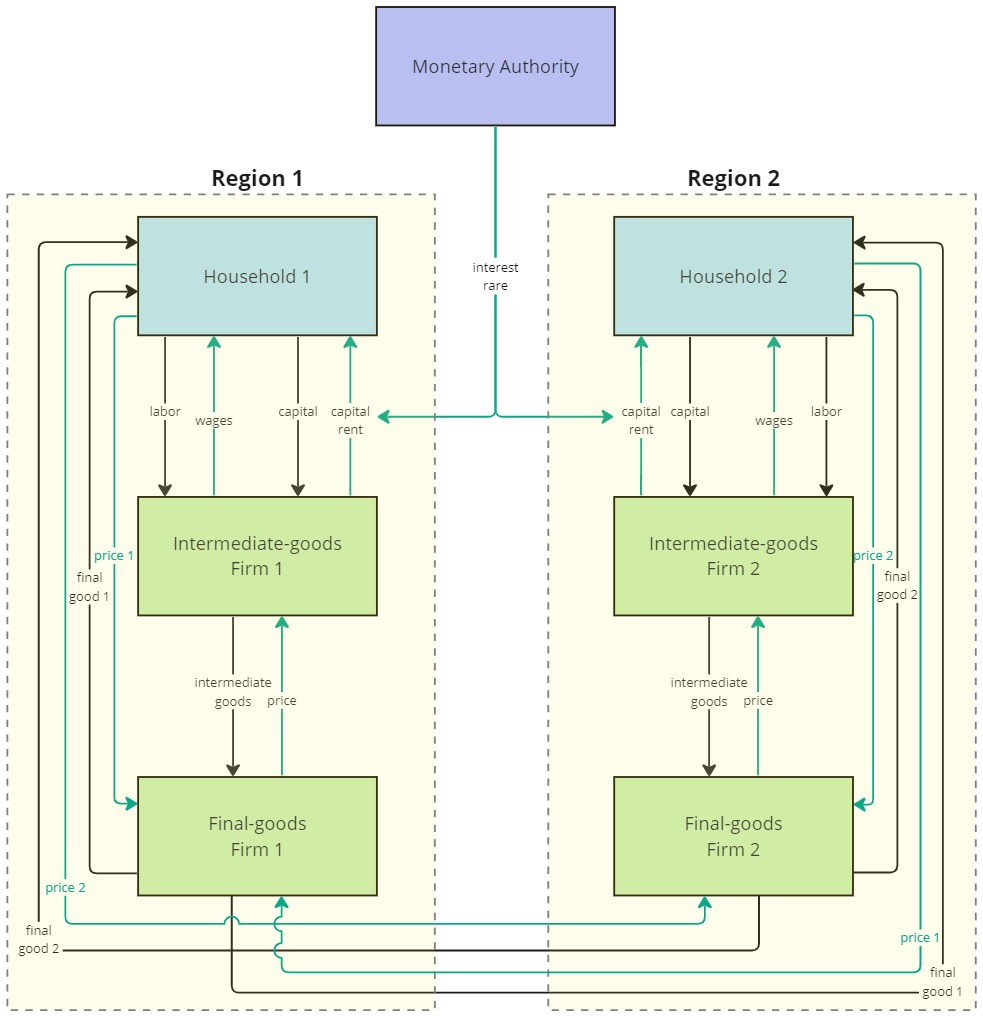
\includegraphics[height=8cm]{flowchart}
		\caption{Model Diagram}
		\label{fig:model-diagram}
		\end{figure}	
		
	\end{frame}

% --------------------------------------------------
% HOUSEHOLD
% --------------------------------------------------

\subsection{Household}

% --------------------------------------------------
% SLIDE
% --------------------------------------------------

\begin{frame}{Cost Minimization Problem}
	
	\begin{align}
	\min_{C_{\eta 1 t}, C_{\eta 2 t}}: &\quad Q_{\eta t} C_{\eta t} = P_{1 t} C_{\eta 1t} + P_{2 t} C_{\eta 2t} \label{eq_v2:reg-consumption-cost}
	\\
	\st: &\quad C_{\eta t} = C_{\eta 1 t}^{\omega_{\eta 1}} C_{\eta 2 t}^{1-\omega_{\eta 1}} \label{eq_v2:reg-consumption-aggregation} \\
	&\quad C_{\eta t} > 0 \nonumber
\end{align}
	
\end{frame}

% --------------------------------------------------
% SLIDE
% --------------------------------------------------

\begin{frame}{Cost Minimization Problem}
	
	Solution:
\begin{align}
	C_{\eta 2 t} &= C_{\eta 1 t} \frac{(1 - \omega_{\eta 1}) P_{1t}}{\omega_{\eta 1} P_{2t}} \label{eq_v2:reg-C-eta-12-t} \\
	C_{\eta 1 t} &= C_{\eta t} \left( \frac{P_{2t} \omega_{\eta 1}}{P_{1t} (1 - \omega_{\eta 1})} \right)^{1-\omega_{\eta 1}} \label{eq_v2:reg-C-eta-1-t} \\
	Q_{\eta t} &= \left( \frac{P_{1 t}}{\omega_{\eta 1}} \right)^{\omega_{\eta 1}} \left( \frac{P_{2 t}}{1 -\omega_{\eta 1}} \right)^{1 -\omega_{\eta 1}} \label{eq_v2:reg-total-expense-level}
\end{align}
	
\end{frame}

% --------------------------------------------------
% SLIDE
% --------------------------------------------------

\begin{frame}{Household Maximization Problem}
	
	\begin{align}
		\max_{C_{\eta t}, L_{\eta t}, K_{\eta,t+1}}: &\quad U_{\eta}(C_{\eta t},L_{\eta t}) = \E \sum_{t=0}^{\infty} \beta^t \left(\frac{C_{\eta t}^{1-\sigma}}{1-\sigma} - \phi \frac{L_{\eta t}^{1+\varphi}}{1+\varphi} \right) \label{eq_v2:reg-utility-function} 
		\\
		\st: &\quad Q_{\eta t} C_{\eta t} + P_{\eta t} I_{\eta t} = W_{\eta t} L_{\eta t} + R_{t} K_{\eta t} + \Pi_{\eta t} \label{eq_v2:reg-budget-constraint} \\
		&\quad K_{\eta,t+1} = (1 - \delta) K_{\eta t} + I_{\eta t} \label{eq_v2:reg-law-of-motion-of-capital} \\
		&\quad C_{\eta t}, L_{\eta t}, K_{\eta t} > 0 \nonumber
	\end{align}
	
\end{frame}

% --------------------------------------------------
% SLIDE
% --------------------------------------------------

\begin{frame}{Household Maximization Problem}
	
	Solution:
\begin{align}
	\frac{\phi L_{\eta t}^{\varphi}}{C_{\eta t}^{-\sigma}} &= \frac{W_{\eta t}}{Q_{\eta t}} \label{eq_v2:reg-labor-supply} \\
	\frac{\mathbb{E}_{t} \{ Q_{\eta,t+1} C_{\eta,t+1}^{\sigma} \} }{ Q_{\eta t} C_{\eta t}^{\sigma} } &= \beta \frac{ \mathbb{E}_{t} \{ P_{\eta,t+1} (1 - \delta) + R_{t+1} \} }{P_{\eta t}} \label{eq_v2:reg-capital-euler-equation}
\end{align}

% Equation \ref{eq_v2:reg-labor-supply}: Household Labor Supply (the marginal rate of substitution (MRS) of labor for consumption is equal to the real wage, which is the relative price between labor and goods).

% Equation \ref{eq_v2:reg-capital-euler-equation}: the Euler equation for the return on capital.
	
\end{frame}

% --------------------------------------------------
% Final-goods Firm
% --------------------------------------------------

\subsection{Final-goods Firm}

% --------------------------------------------------
% SLIDE
% --------------------------------------------------

\begin{frame}{Final-goods Firm Maximization Problem}
	
\begin{align}
	\max_{Y_{\eta jt}}: &\quad P_{\eta t} Y_{\eta t} - \int_{0}^{1} P_{\eta jt} Y_{\eta jt} \dif j \label{eq_v2:reg-final-goods-firm-max-problem} \\
	\st: & \quad Y_{\eta t} = \left( \int_{0}^{1} Y_{\eta jt}^{\frac{\psi-1}{\psi}} \dif j \right)^{\frac{\psi}{\psi-1}} \label{eq_v2:reg-final-goods-firm-bundle-rule}
\end{align}
	
\end{frame}

% --------------------------------------------------
% SLIDE
% --------------------------------------------------

\begin{frame}{Final-goods Firm Maximization Problem}
	
Solution:
\begin{align}
	Y_{\eta jt} &= Y_{t} \left( \frac{P_{\eta t}}{P_{\eta jt}} \right)^{\psi} \label{eq_v2:reg-final-goods-firm-FOC} \\
	P_{\eta t} & = \left[ \int_{0}^{1} P_{\eta jt}^{1-\psi} \dif j \right]^{\frac{1}{1-\psi}} \label{eq_v2:reg-final-goods-firm-markup}
\end{align}

%Equation \ref{eq_v2:reg-final-goods-firm-FOC} shows that the demand for variety $j$ depends on its relative price.

%Equation \ref{eq_v2:reg-final-goods-firm-markup} is the final-goods firm's markup.
	
\end{frame}

% --------------------------------------------------
% Intermediate-goods Firm
% --------------------------------------------------

\subsection{Intermediate-goods Firm}

% --------------------------------------------------
% SLIDE
% --------------------------------------------------

	\begin{frame}{Intermediate-goods Firm Problems}
		
	\begin{align}
		\label{eq_v2:reg-int-good-firm-total-cost}
		\min_{K_{\eta jt}, L_{\eta jt}}: \quad & R_{t} K_{\eta jt} + W_t L_{\eta jt} \\
		\label{eq_v2:reg-int-good-firm-prod-function}
		\st: \quad & Y_{\eta jt} = Z_{A\eta t} K_{\eta jt}^{\alpha_{\eta}} L_{\eta jt}^{1-{\alpha_{\eta}}}
	\end{align}
				
	\end{frame}

% --------------------------------------------------
% SLIDE
% --------------------------------------------------

\begin{frame}{Intermediate-goods Firm Problems}

Solutions:
\begin{align}
	\frac{K_{\eta jt}}{L_{\eta jt}} &= \left( \frac{{\alpha_{\eta}}}{1-\alpha_{\eta}} \right) \frac{W_{\eta t}}{R_{t}} \label{eq_v2:reg-int-good-firm-TMRS} \\
	K_{\eta jt} & = \frac{Y_{\eta jt}}{Z_{A\eta t}} \left[ \left( \frac{{\alpha_{\eta}}}{1-\alpha_{\eta}} \right) \frac{W_{\eta t}}{R_{t}}\right]^{1-\alpha_{\eta}} \label{eq_v2:reg-int-good-firm-Kt-demand} \\
	L_{\eta jt} & = \frac{Y_{\eta jt}}{Z_{A\eta t}} \left[ \left( \frac{{\alpha_{\eta}}}{1-\alpha_{\eta}} \right) \frac{W_{\eta t}}{R_{t}}\right]^{-{\alpha_{\eta}}} \label{eq_v2:reg-int-good-firm-Lt-demand} \\
	\Lambda_{\eta t} &= \frac{1}{Z_{A\eta t}} \left( \frac{R_{t}}{{\alpha_{\eta}}} \right)^{{\alpha_{\eta}}} \left( \frac{W_{\eta t}}{1-\alpha_{\eta}} \right)^{1-\alpha_{\eta}} \label{eq_v2:reg-int-good-firm-MC-2}
\end{align}

\end{frame}

\begin{comment}
	
	\begin{alignat}{2}
		TC_{\eta jt} & = \frac{Y_{\eta jt}}{Z_{A\eta t}} \left( \frac{R_{t}}{{\alpha_{\eta}}} \right)^{{\alpha_{\eta}}} \left( \frac{W_{\eta t}}{1-\alpha_{\eta}} \right)^{1-\alpha_{\eta}} \label{eq_v2:reg-int-good-firm-TC}
	\end{alignat}
	
	% Equation \ref{eq_v2:reg-int-good-firm-TMRS} demonstrates the relationship between the technical marginal rate of substitution (TMRS) and the economic marginal rate of substitution (EMRS). 
	
	% Equation \ref{eq_v2:reg-int-good-firm-Kt-demand} is the intermediate-goods firm demand for capital. 
	
	% Equation \ref{eq_v2:reg-int-good-firm-Lt-demand} is the intermediate-goods firm demand for labor.
	
	% Equation \ref{eq_v2:reg-int-good-firm-TC} is the intermediate-goods firm total cost.
	
	% Equation \ref{eq_v2:reg-int-good-firm-MC-2} is the intermediate-goods firm marginal cost.
	
\end{comment}

% --------------------------------------------------
% SLIDE
% --------------------------------------------------

\begin{frame}{Intermediate-goods Firm Problems}
	
	Price Stickiness and Profit Flow, Calvo's Rule \cite{calvo_staggered_1983}:
\begin{align}
	\label{eq_v2:reg-int-good-firm-optimal-price-problem}
	\max_{P_{\eta jt}}: & \quad \E \sum_{s=0}^{\infty} \left\{ \frac{ \theta^s \left[ P_{\eta jt} Y_{\eta j,t+s} - TC_{\eta j,t+s} \right]}{\prod_{k=0}^{s-1}(1+R_{t+k})} \right\} \\
	\tag{\ref{eq_v2:reg-final-goods-firm-FOC}}
	\st: & \quad Y_{\eta jt} = Y_{\eta t} \left( \frac{P_{\eta t}}{P_{\eta jt}} \right)^{\psi}
\end{align}
	
\end{frame}

% --------------------------------------------------
% SLIDE
% --------------------------------------------------

\begin{frame}{Intermediate-goods Firm Problems}
	
	Solution:
	\begin{align}
		P_{\eta t}^{\ast} &= \frac{\psi}{\psi-1} \cdot \frac{\E \sum_{s=0}^{\infty} \left\{ \theta^s Y_{\eta j,t+s} \Lambda_{\eta, t+s} / \prod_{k=0}^{s-1}(1+R_{t+k}) \right\}}{\E \sum_{s=0}^{\infty} \left\{ \theta^s Y_{\eta j,t+s} / \prod_{k=0}^{s-1}(1+R_{t+k}) \right\}} \label{eq_v2:reg-int-good-firm-optimal-price-FOC-3} \\
		P_{\eta t} & = \left[ \theta P_{\eta, t-1}^{1-\psi} + (1-\theta) P_{\eta t}^{\ast 1-\psi} \right]^\frac{1}{1-\psi} \label{eq_v2:reg-general-price-level}
	\end{align}
	
\end{frame}


% --------------------------------------------------
% REGIONAL INFLATION
% --------------------------------------------------

\begin{frame}{Regional Inflation}

\subsubsection{Regional Inflation}

\begin{align}
	\pi_{\eta t} = \frac{P_{\eta t}}{P_{\eta, t-1}} \label{eq_v2:reg-regional-inflation}
\end{align}

\end{frame}

% --------------------------------------------------
% SLIDE
% --------------------------------------------------

\subsection{Monetary Authority}

\begin{frame}{Monetary Authority}
	
Taylor's Rule \cite{taylor_discretion_1993}:	
\begin{align}
	\frac{R_{t}}{R} &= \left( \frac{R_{t-1}}{R} \right)^{\gamma_{R}}  \left[\left( \frac{\pi_t}{\pi} \right)^{\gamma_{\pi}} \left( \frac{Y_{t}}{Y} \right)^{\gamma_{Y}} \right]^{1-\gamma_{R}} Z_{Mt} \label{eq_v2:reg-monetary-policy} \\
	&\quad \text{where: } \pi_{t} = \pi_{1t}^{\theta_{\pi}} \pi_{2t}^{1 - \theta_{\pi}} \label{eq_v2:reg-gross-inflation-rate} \\ 
	&\quad \text{and: } \theta_{\pi} = \frac{P_{1t} Y_{1t}}{P_{1t} Y_{1t} + P_{2t} Y_{2t}} \label{eq_v2:reg-theta-pi}
\end{align}
	
	
\end{frame}

% --------------------------------------------------
% SLIDE
% --------------------------------------------------

\subsection{Stochastic Shocks}

\begin{frame}{Stochastic Shocks}
	
	Productivity Shock:
	\begin{align}
		\ln{Z_{At}} = (1-\rho_A)\ln{Z_A} + \rho_A\ln{Z_{A,t-1}} + \varepsilon_{At} \label{eq:productivity-shock}
	\end{align}
	
	Monetary Policy Shock:
	\begin{align}
		\ln{Z_{Mt}} &= (1-\rho_M)\ln{Z_{M}} + \rho_M\ln{Z_{M,t-1}} + \varepsilon_{Mt} \label{eq:monetary-shock}
	\end{align}
	
\end{frame}

% --------------------------------------------------
% Equilibrium Conditions
% --------------------------------------------------

\subsection{Equilibrium Conditions}

\begin{frame}{Equilibrium Conditions}
	
A Competitive Equilibrium consists of sequences of:

- prices $\{P_{\eta t}^{\ast}, R_t^{\ast}, W_{\eta t}^{\ast}\}$, 

- allocations for households $\mathbfscr{A}_H \coloneq \{C_{\eta 1 t}^{\ast}, C_{\eta 2 t}^{\ast}, L_{\eta t}^{\ast}, I_{\eta t}^{\ast}, K_{\eta, t+1}^{\ast}\}$ 

- allocations for firms $\mathbfscr{A}_F \coloneq \{K_{\eta jt}^{\ast}, L_{\eta jt}^{\ast}, Y_{\eta jt}^{\ast}, Y_{\eta t}^{\ast}\}$. 

In such an equilibrium, given the set of exogenous variables $\{K_0, Z_{A\eta t}, Z_{Mt}\}$, the elements in $\mathbfscr{A}_H$ solve the household problem, while the elements in $\mathbfscr{A}_F$ solve the firms' problems, and the markets for goods and labor clear:
\begin{align}
	& Y_{t} = Y_{1 t} + Y_{2 t} \label{eq_v2:reg-market-clearing-condition-Yt} \\
	%& \quad \text{where:} \quad Y_{\eta t} = C_{\eta t} + I_{\eta t} \label{eq_v2:reg-regional-demand} \\
	& L_{\eta t} = \int_{0}^{1} L_{\eta jt} \dif j \label{eq_v2:reg-market-clearing-condition-Lt} 
\end{align}
	
\end{frame}

% --------------------------------------------------
% SLIDE
% --------------------------------------------------

\subsection{Steady State}

\begin{frame}{Steady State}
	
	\centering \huge Steady State
	
\end{frame}

% --------------------------------------------------
% SLIDE
% --------------------------------------------------

\begin{frame}{Steady State}
	
	Steady state solution \cite[p.41]{costa_junior_understanding_2016}:
	\begin{align}
		\mathbb{E}_t X_{t+1} = X_t = X_{t-1} = X_{ss}
	\end{align}
		
\end{frame}

% --------------------------------------------------
% SLIDE
% --------------------------------------------------

\subsection{Log-linearization}

\begin{frame}{Log-linearization}
	
	\centering \huge Log-linearization
		
\end{frame}

% --------------------------------------------------
% SLIDE
% --------------------------------------------------

\begin{frame}{Log-linearization}
	
	Uhlig's rules for log-linearization \cite{uhlig_toolkit_1999}.
	
	\begin{align*}
		\hat{x}_t \coloneqq \frac{x_t - x}{x} \iff x_t = x(1 + \hat{x}_t)
	\end{align*}	
	
\end{frame}

% --------------------------------------------------
% SLIDE
% --------------------------------------------------

\subsection{Log-linear Model}

\begin{frame}[allowframebreaks]{Log-linear Model}

Square system of 30 variables and equations:
	
\begin{itemize}
	
	\item Real Variables: $\langle \begin{matrix} \hat{C}_{\eta } & \hat{L}_{\eta } & \hat{K}_{\eta} & \hat{I}_{\eta} & \hat{C}_{\eta 1} & \hat{C}_{\eta 2} & \hat{Y}_{\eta } & \hat{Y}_{} & \hat{Z}_{A\eta } & \hat{Z}_{M} \end{matrix} \rangle$;
	
	\item Nominal Variables: $\langle \begin{matrix} \hat{Q}_{\eta} & \hat{P}_{\eta } & \hat{R}_{} & \hat{\pi}_{} & \hat{W}_{\eta } & \hat{\lambda}_{\eta } & \hat{\pi}_{\eta } \end{matrix} \rangle$.
	
\end{itemize}
	
\end{frame}

% --------------------------------------------------
% SLIDE
% --------------------------------------------------

\begin{frame}[allowframebreaks]{Log-linear Model}
	
{\singlespacing
		
	\begin{itemize}
		
		\item Regional Gross Inflation Rate
		\begin{align}
			\hat{\pi}_{\eta t} &= \hat{P}_{\eta t} - \hat{P}_{\eta, t-1} \label{eq_v2:level-dev-regional-inflation}
		\end{align}
		
		\item New Keynesian Phillips Curve
		\begin{align}
			\hat{\pi}_{\eta t} &= \beta \E \hat{\pi}_{\eta, t+1} + \frac{(1-\theta) (1- \theta \beta)}{\theta} \hat{\lambda}_{\eta t} \label{eq_v2:reg-nk-phillips-curve-mc}
		\end{align}
		
		\item Regional Consumption Weight
		\begin{align}
			\hat{C}_{\eta 2t} - \hat{C}_{\eta 1t} &= \hat{P}_{1t} - \hat{P}_{2t} \label{eq_v2:reg-C-eta-12-t-ll}
		\end{align}
		
		\item Regional Consumption of Good 1
		\begin{align}
			\hat{C}_{\eta t} - \hat{C}_{\eta 1 t} &= (1 - \omega_{\eta 1}) (\hat{P}_{1t} - \hat{P}_{2t}) \label{eq_v2:reg-C-eta-1-t-ll}
		\end{align}
		
		\item Regional Price Index
		\begin{align}
			\hat{Q}_{\eta t} &= \omega_{\eta 1} \hat{P}_{1 t} + (1 -\omega_{\eta 1}) \hat{P}_{2 t} \label{eq_v2:reg-total-expense-level-ll}
		\end{align}
		
		\item Labor Supply
		\begin{alignat}{2}
			\varphi \hat{L}_{\eta t} + \sigma \hat{C}_{\eta t} &= \hat{W}_{\eta t} - \hat{Q}_{\eta t} \label{eq_v2:reg-ll-labor-supply}
		\end{alignat}
		
		\item Law of Motion for Capital
		\begin{align}
			\hat{K}_{\eta, t+1} &= (1-\delta) \hat{K}_{\eta t} + \delta \hat{I}_{\eta t} \label{eq_v2:reg-ll-law-of-motion-for-capital}
		\end{align}
		
		\item Euler equation for capital return
		\begin{align}
			\begin{split}
				(\hat{Q}_{\eta, t+1} - \hat{Q}_{\eta t}) + \sigma(\hat{C}_{\eta, t+1} - \hat{C}_{\eta t}) - (\hat{P}_{\eta, t+1} - \hat{P}_{\eta, t}) = \\
				\qquad = \beta r_{}(\hat{R}_{\eta, t+1} - \hat{P}_{\eta, t+1})
			\end{split} \label{eq_v2:reg-ll-capital-euler-equation}
		\end{align}
		
		\item Production Function
		\begin{align}
			\hat{Y}_{\eta t} &= \hat{Z}_{A\eta t} + {\alpha_{\eta}} \hat{K}_{\eta t} + (1-\alpha_{\eta}) \hat{L}_{\eta t} \label{eq_v2:reg-ll-final-goods-firm-bundle-rule-3}
		\end{align}
		
		\item Technical and Economic Marginal Rates of Substitution % (TMRS and EMRS)
		\begin{align}
			\hat{K}_{\eta t} - \hat{L}_{\eta t} &= \hat{W}_{\eta t} - \hat{R}_{t} \label{eq_v2:reg-ll-int-good-firm-TMRS}
		\end{align}
		
		\item Marginal Cost
		\begin{align}
			\hat{\lambda}_{\eta t} &= {\alpha_{\eta}} \hat{R}_{t} + (1- {\alpha_{\eta}}) \hat{W}_{\eta t} - \hat{Z}_{A\eta t} - \hat{P}_{\eta t} \label{eq_v2:reg-ll-int-good-firm-MC-3}
		\end{align}
		
		\item Monetary Policy
		\begin{align}
			\hat{R}_t = \gamma_{R} \hat{R}_{t-1} + (1-\gamma_{R})(\gamma_{\pi} \hat{\pi}_t + \gamma_{Y} \hat{Y}_t) + \hat{Z}_{Mt} \label{eq_v2:reg-ll-monetary-policy}
		\end{align}
		
		\item National Gross Inflation Rate
		\begin{align}
			\hat{\pi}_{t} &= \theta_{\pi} \hat{\pi}_{1t} + (1 - \theta_{\pi}) \hat{\pi}_{2t} \label{eq_v2:reg-gross-inflation-rate-ll}
		\end{align}
		
		\item Productivity Shock
		\begin{alignat}{2}
			\hat{Z}_{A\eta t} &= \rho_{A\eta} \hat{Z}_{A\eta, t-1} + \varepsilon_{A\eta} \label{eq_v2:reg-ll-productivity-shock}
		\end{alignat}
		
		\item Monetary Shock
		\begin{alignat}{2}
			\hat{Z}_{Mt} &= \rho_M \hat{Z}_{M,t-1} + \varepsilon_{M} \label{eq_v2:reg-ll-monetary-shock}
		\end{alignat}
		
		\item Goods-Market Clearing Condition
		\begin{align}
			\hat{Y}_{t} &= \theta_{Y} \hat{Y}_{1t} + (1-\theta_{Y}) \hat{Y}_{2t} \label{eq_v2:reg-ll-market-clearing-condition-Yt-3}
		\end{align}
		
		\item Regional Goods-Market Clearing Condition
		\begin{align}
			\hat{Y}_{\eta t} &= \theta_{C\eta} \hat{C}_{\eta t} + (1 - \theta_{C\eta}) \hat{I}_{\eta t} \label{eq_v2:reg-ll-total-yn-2}
		\end{align}
		
	\end{itemize}
	
} %\singlespacing
	
\end{frame}

\begin{comment}

% --------------------------------------------------
% SLIDE
% --------------------------------------------------

\subsection{Matlab and Dynare}

\begin{frame}{Matlab and Dynare}
	
	\begin{figure}[h!]
		\centering
		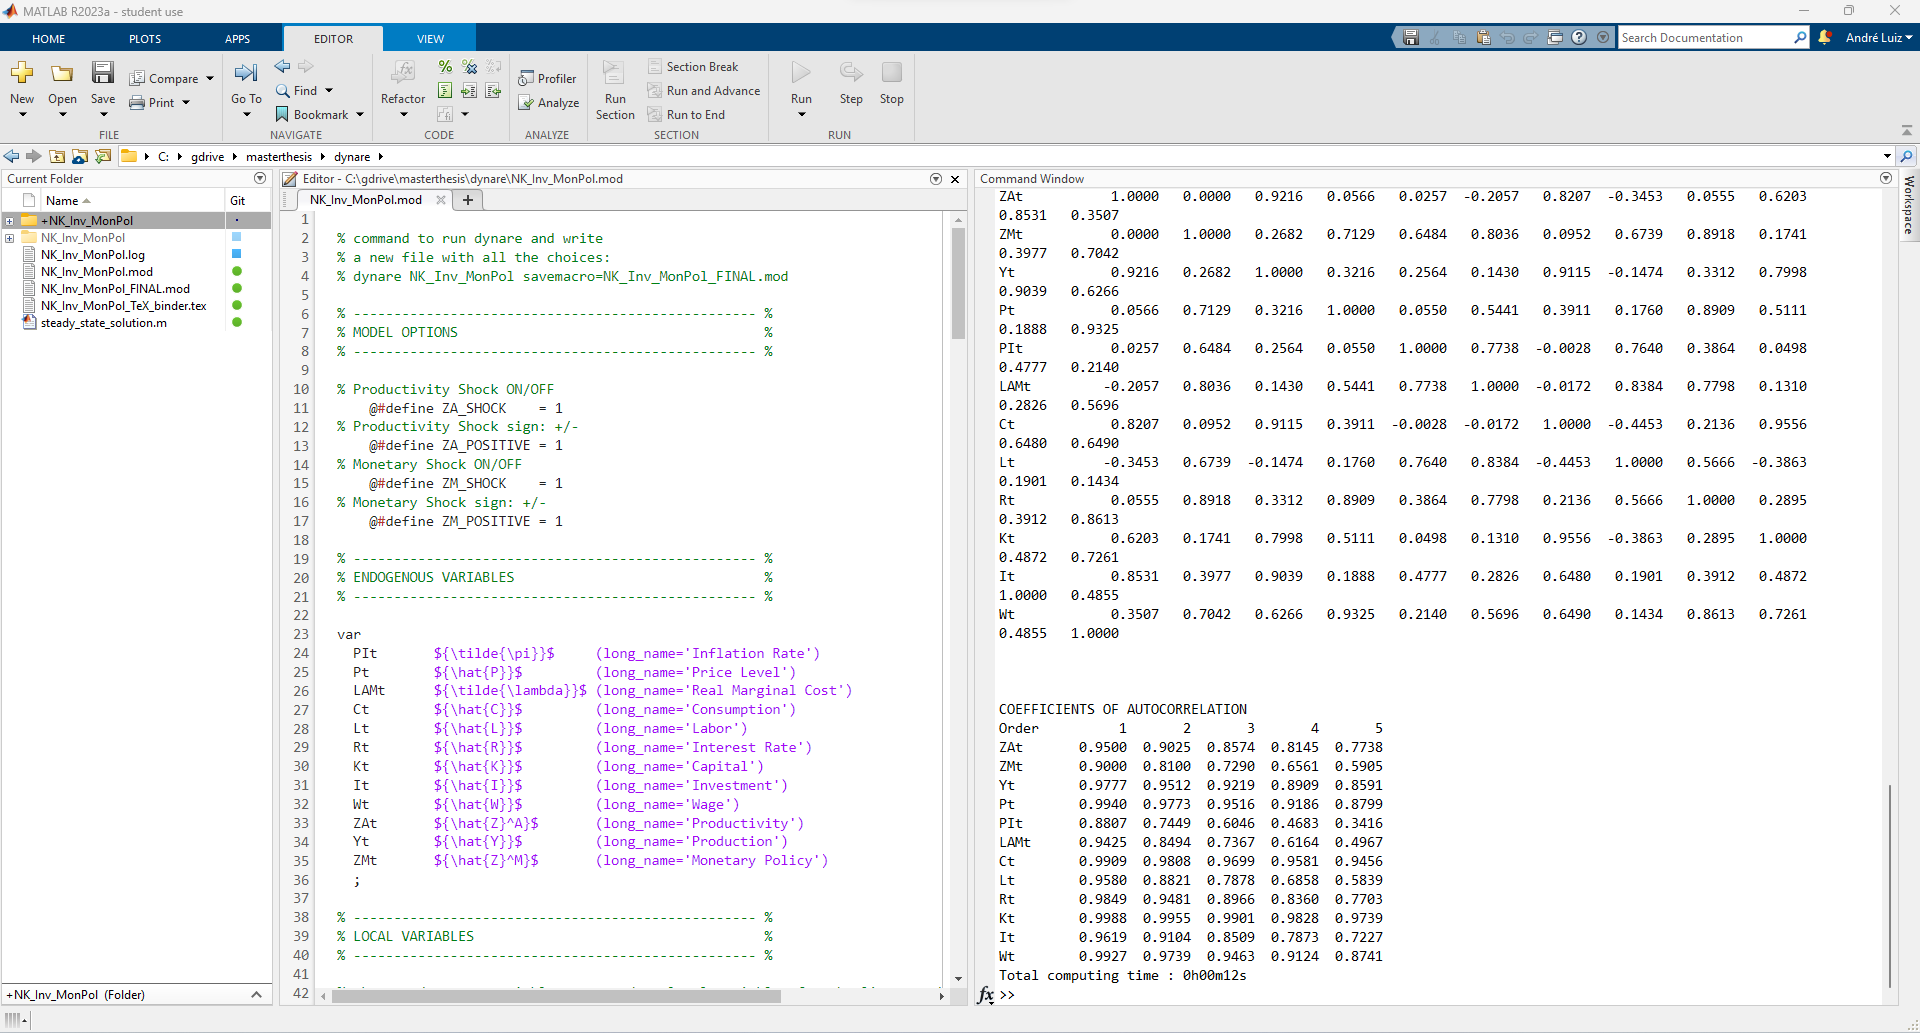
\includegraphics[width=\textwidth]{matlab_screen}
		\caption{Matlab and Dynare}
		\label{fig:matlab}
	\end{figure}
	
\end{frame}
	
\end{comment}

\end{document}